%Latex for Astro301 Homework 1
%Astro301 Spring 2018
%Author: Chase Urasaki
%Created: 2.7.2018
%Updated: 2.8.2018

%%%%%%%%%%%%%%%%%%%%%%%%%%%%%%%%%%%%%%%%%%%%%%%%%%%%%%%%%%%%%%%%
\documentclass[12pt]{article}
\usepackage{graphicx}
\usepackage{float}
\usepackage{indentfirst}
\usepackage{amssymb}

\begin{document} 

\title{Homework 1: Galaxy SEDs, Filters, and Photometric Redshifts}
\author{Chase Urasaki}

\date{\today}

\maketitle 

\section{Part 1}
\begin{center}
\begin{figure}[H]
\label{SEDs}
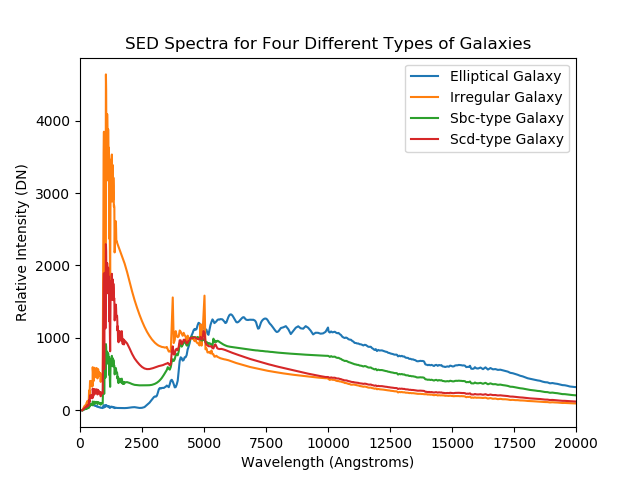
\includegraphics[scale=1.0]{SEDs.png}
\caption{Spectral Energy Distributions (SEDs) for each of the four galaxies that we were given. The fluxes were given in arbitrary units, while the wavelengths are given in Angstroms}. 
\end{figure}
\end{center}

\begin{center}
\begin{figure}[H]
\label{Filter_Curves}
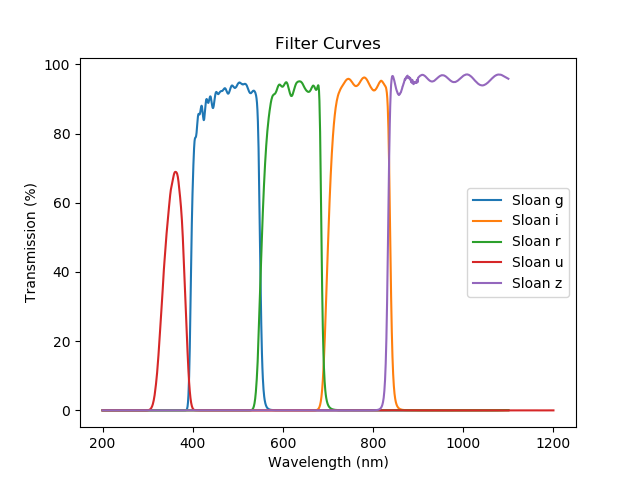
\includegraphics[scale=0.5]{Filter_curves.png}
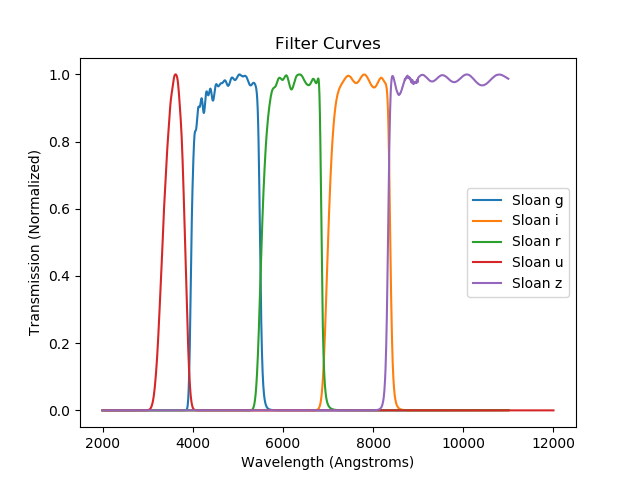
\includegraphics[scale=0.5]{Filter_curves_norm.png}
\caption{This is the Plot for the filter curve values. The  plot on the left is a plot of the raw data. The plot on the right is normalized and the wavelengths have been changed to Angstroms.}
\end{figure}
\end{center}

\section{Part 2}
Below is a table for the Galaxy type and computed colors at redshift 0. 
%%Create the table for the color values
\begin{center}
 \begin{tabular}{||c c c c c||} 
 \hline
 Galaxy Type & u'-g' & g'-r' & r'-i' & i'-z' \\ [0.5ex] 
 \hline\hline
 Elliptical & 2.37 & 0.09 & -0.04 & 0.63 \\ 
 \hline
 Irregular & 1.20 & -0.52 & -0.19 & 0.50 \\
 \hline
 Sbc & 1.71 & -0.21 & -0.05 & 0.63\\
 \hline
 Scd & 1.54 & -0.33 & -0.20 & 0.43 \\
 \hline
\end{tabular}
\end{center}

At redshift zero, the Sloan g' filter can best determine the type of galaxy, from the images below, each galaxy has a very distinct Sloan g' transmission curve. 

\begin{center}
	\begin{figure}[H]
	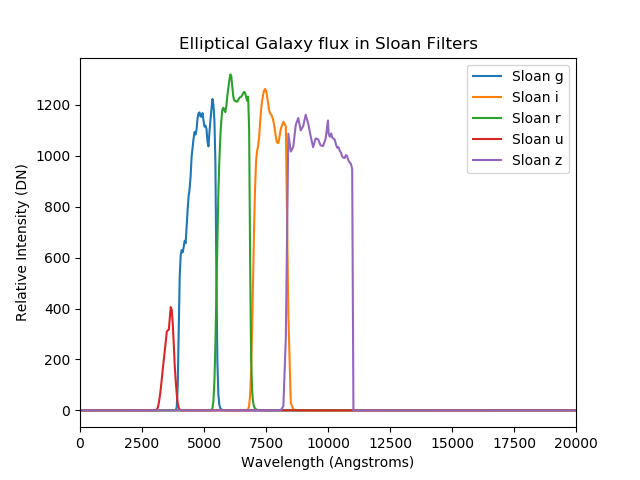
\includegraphics[scale=0.5]{El_sloan.png}
	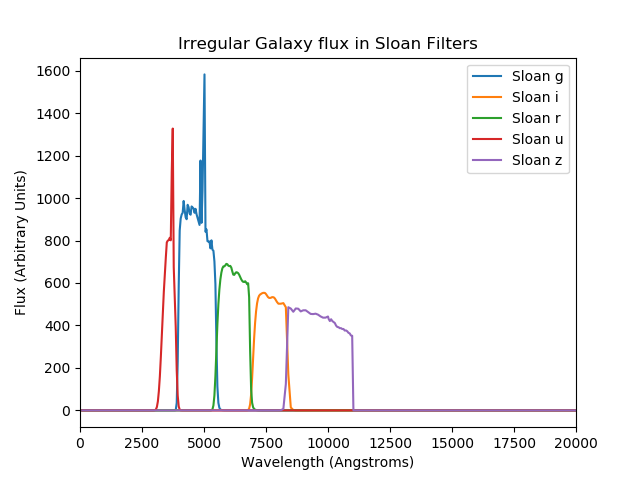
\includegraphics[scale=0.5]{Irr_sloan.png}
	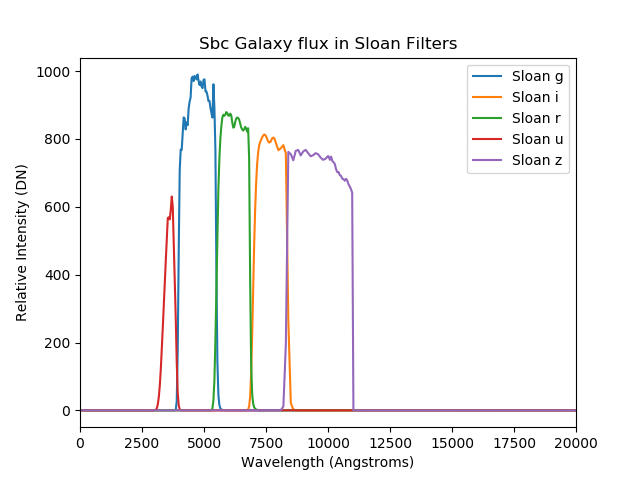
\includegraphics[scale=0.5]{Sbc_sloan.png}
	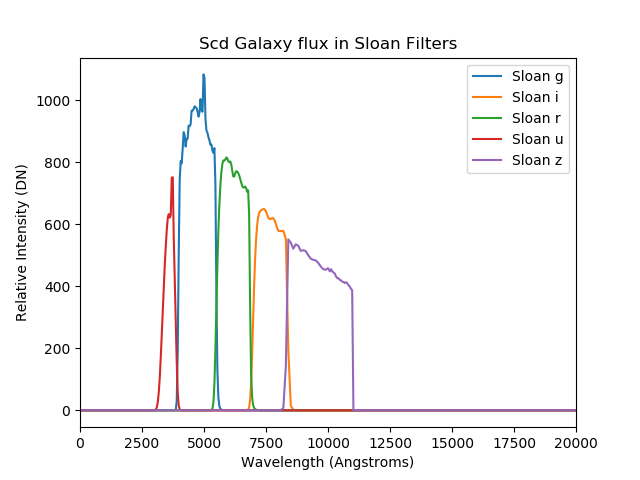
\includegraphics[scale=0.5]{Scd_sloan.png}
	\end{figure}
\end{center}

A galaxy's color is essentially an indicator of the difference in red or blue in each of the respective filter differences. For 'redder' galaxies, we can expect that much of the stellar population includes dwarf stars and older stars such as red giants. The distinction for 'bluer' galaxies isn't quite so clear however. While a galaxies color may be more blue, that means that it contains younger, hotter, and more luminous stars. However, the stellar popution could be the dominated by older stars are less luminous than their younger counterparts. 

\section{Part 3}
Recall that the redshift is defined as $\lambda_{observed} = \lambda_{rest} (1 + z)$. 
Below are the color vs. color diagrams.
\begin{center}
	\begin{figure}[H]
	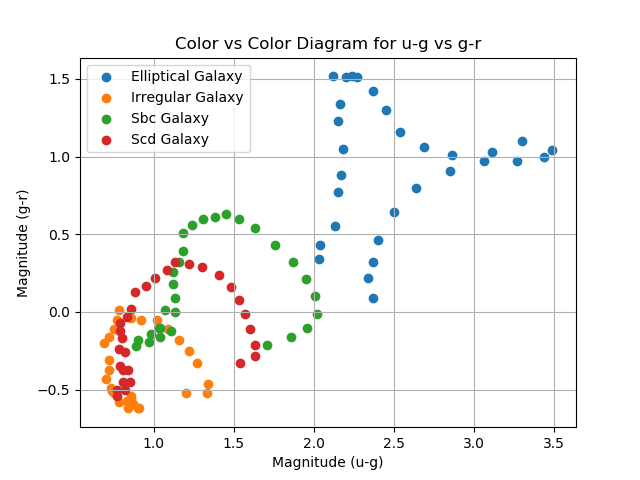
\includegraphics[scale=1.0]{u_g_vs_g_r.png}
	\caption{Color vs. color diagram for the g-r vs r-i magnitudes.}
	\end{figure}
	
	\begin{figure}
	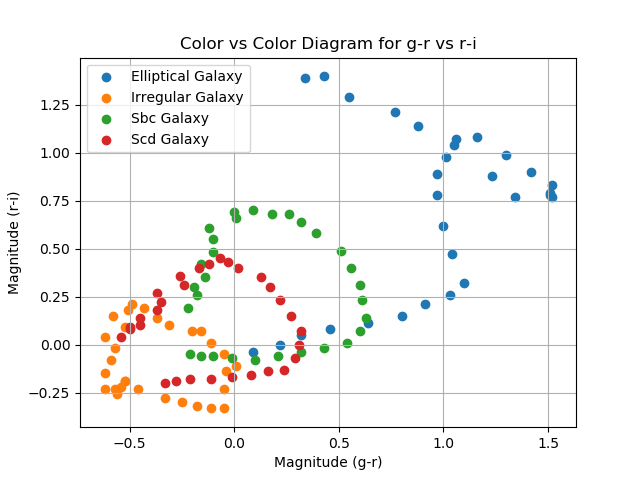
\includegraphics[scale=1.0]{g_r_vs_r_i.png}
	\caption{Color vs color diagram for the g-r vs r-i magnitudes.}
	\end{figure}
	
	\begin{figure}[H]
	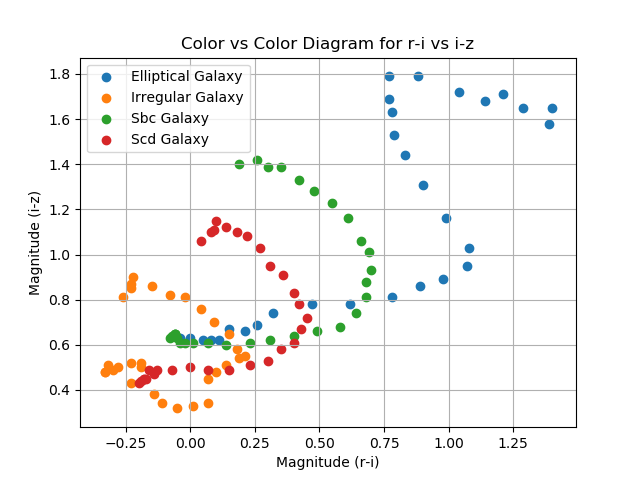
\includegraphics[scale=1.0]{r_i_vs_i_z.png}
	\caption{Color vs color diagram for the r-i vs i-z magnitudes.}
	\end{figure}
\end{center}

If we wanted to visulaize the redshifts as well, one way to do that is to create another axis that comes out of the page to represent z values. This would create a three dimensional plot that you could intuitively understand as points with larger z values will be further 'into the page'. 
\end{document}